\subsubsection{完整工程：组织文件并生成消息接口}
\label{sec:ros2-project}
刚才我们逐段写了节点和消息接口，现在把它们拼成一个能运行的小工程。完整源码就在本卷 \path{examples/ros2/basic-interfaces-demo}，包括两个包。my\_msgs 先生成消息类型，my\_package 再使用它；文件之间的关系如下：
\par\medskip\noindent\begin{minipage}{\linewidth}
\begin{lstlisting}[language={}]
basic-interfaces-demo/
  README.md
  my_msgs/
    CMakeLists.txt
    package.xml
    msg/My.msg
  my_package/
    CMakeLists.txt
    package.xml
    include/my_package/my_node.h
    src/my_node.cpp
    src/node_run.cpp
\end{lstlisting}
\end{minipage}\par\smallskip
你可以照着下面写，也可以把两个包复制到新工作空间的 src 中，再逐个核对。

\begin{example}[准备消息包与接口生成规则]
首先准备消息包。这个文件只写字段，不写 C++ 类定义，构建工具会自动生成代码。
\par\medskip\noindent\begin{minipage}{\linewidth}
\lstinputlisting[frame=single,language={},caption={my\_msgs/msg/My.msg}]{examples/ros2/basic-interfaces-demo/my_msgs/msg/My.msg}
\end{minipage}\par\smallskip

下面两份文件让 ROS2 知道“要生成哪个接口、依赖哪些类型”。std\_msgs 提供 Header，rosidl 提供接口代码生成过程；这两项都要先安装好。
\par\medskip\noindent\begin{minipage}{\linewidth}
\lstinputlisting[frame=single,language=cmake,label=lst:cmake_2,caption={my\_msgs/CMakeLists.txt}]{examples/ros2/basic-interfaces-demo/my_msgs/CMakeLists.txt}
\end{minipage}\par\smallskip
\par\medskip\noindent\begin{minipage}{\linewidth}
\lstinputlisting[frame=single,language=XML,label=lst:xml_2,caption={my\_msgs/package.xml}]{examples/ros2/basic-interfaces-demo/my_msgs/package.xml}
\end{minipage}\par\smallskip

\end{example}

\Needspace{35\baselineskip}
\subsubsection{完整工程：实现节点并声明构建依赖}
\begin{example}[把发布、订阅和定时器接起来]
接下来准备节点包。头文件声明节点类并保存发布者、订阅者和定时器句柄；把句柄放在成员中，节点运行时它们才会一直存活。
\par\medskip\noindent\begin{minipage}{\linewidth}
\lstinputlisting[frame=single,language=C++,label=lst:my_node_h,caption={my\_package/include/my\_package/my\_node.h},numbers=left,numberstyle={\color{gray}\tiny}]{examples/ros2/basic-interfaces-demo/my_package/include/my_package/my_node.h}
\end{minipage}\par\smallskip

实现文件中的构造函数先创建各个接口并绑定回调。收到 receive 后，字符串回调把内容加上前缀发到 send；定时器每秒发布一次计数和自定义消息。节点还订阅自己的 my\_msg，方便你在日志里看见字段确实经过了通信。
\lstinputlisting[frame=single,language=C++,lastline=52,label=lst:my_node_cpp,caption={my\_package/src/my\_node.cpp},numbers=left,numberstyle={\color{gray}\tiny}]{examples/ros2/basic-interfaces-demo/my_package/src/my_node.cpp}
定时器回调再填入时间戳、坐标系和检测结果，然后发布消息。下面接着展示同一文件，行号保持连续：
\par\medskip\noindent\begin{minipage}{\linewidth}
\lstinputlisting[frame=single,language=C++,firstline=53,firstnumber=53,lastline=68,caption={my\_node.cpp 的定时器回调},numbers=left,numberstyle={\color{gray}\tiny}]{examples/ros2/basic-interfaces-demo/my_package/src/my_node.cpp}
\end{minipage}\par\smallskip

\Needspace{9\baselineskip}
文件最后的自订阅回调只负责打印字段。这样我们不用再写第二个节点，也能先检查自定义消息是否按约定传了过来：
\par\medskip\noindent\begin{minipage}{\linewidth}
\lstinputlisting[frame=single,language=C++,firstline=69,firstnumber=69,caption={my\_node.cpp 的自定义消息回调},numbers=left,numberstyle={\color{gray}\tiny}]{examples/ros2/basic-interfaces-demo/my_package/src/my_node.cpp}
\end{minipage}\par\smallskip


最后由入口文件初始化 ROS2、创建节点并调用 spin。spin 让执行器调度回调。如果只创建对象却不进入执行器，回调不会按上面的预期工作。
\par\medskip\noindent\begin{minipage}{\linewidth}
\lstinputlisting[frame=single,language=C++,label=lst:node_run_cpp,caption={my\_package/src/node\_run.cpp},numbers=left,numberstyle={\color{gray}\tiny}]{examples/ros2/basic-interfaces-demo/my_package/src/node_run.cpp}
\end{minipage}\par\smallskip

节点包的构建规则显式找到 rclcpp、std\_msgs 和刚才的 my\_msgs，创建 my\_node 目标，并把它安装到 ROS2 能查到的位置。包清单中的 my\_msgs 依赖也让 colcon 能按正确顺序构建两个包。
\par\medskip\noindent\begin{minipage}{\linewidth}
\lstinputlisting[frame=single,language=cmake,label=lst:ros2-basic-cmake,caption={my\_package/CMakeLists.txt}]{examples/ros2/basic-interfaces-demo/my_package/CMakeLists.txt}
\end{minipage}\par\smallskip
\Needspace{19\baselineskip}
\par\medskip\noindent\begin{minipage}{\linewidth}
\lstinputlisting[frame=single,language=XML,label=lst:xml_1,caption={my\_package/package.xml}]{examples/ros2/basic-interfaces-demo/my_package/package.xml}
\end{minipage}\par\smallskip

\end{example}

\subsubsection{完整工程：编译并验证话题收发}
\begin{example}[先生成接口，再启动节点]
把两个包放进 \path{~/ros2_ws/src} 后，回到工作空间根目录构建。
\par\medskip\noindent\begin{minipage}{\linewidth}
\begin{tbash}
source /opt/ros/humble/setup.bash
cd ~/ros2_ws
colcon build --packages-up-to my_package
source install/setup.bash
ros2 run my_package my_node
\end{tbash}
\end{minipage}\par\smallskip
\texttt{--packages-up-to} 同时构建工作空间中的消息依赖。节点应每秒记录一次 timer count，并打印 id 为 1、yaw 为 0.25 的自定义消息。

终端二加载同一系统与工作空间环境后观察一次消息：
\par\medskip\noindent\begin{minipage}{\linewidth}
\begin{tbash}
source /opt/ros/humble/setup.bash
source ~/ros2_ws/install/setup.bash
ros2 topic echo /my_msg --once
ros2 topic echo /timer_ --once
ros2 topic echo /send
\end{tbash}
\end{minipage}\par\smallskip
先保持 send 的观察进程运行，再开一个同样加载环境的终端发送：
\par\medskip\noindent\begin{minipage}{\linewidth}
\begin{tbash}
ros2 topic pub --once /receive std_msgs/msg/String "{data: hello}"
\end{tbash}
\end{minipage}\par\smallskip
节点日志应显示收到 hello，send 应收到 I can hear:hello。按 Ctrl+C 结束节点和观察进程，再修改代码做练习。
\end{example}

\subsubsection{用 rqt 发布输入与监视回复}
\begin{example}[用 rqt 看见同一条消息经过了哪里]
终端里的收发已经跑通了，我们再把它搬到图形界面。先让 my\_node 保持运行，在同样加载了环境的两个终端分别打开插件：
\par\medskip\noindent\begin{minipage}{\linewidth}
\begin{tbash}
ros2 run rqt_gui rqt_gui --standalone rqt_publisher
ros2 run rqt_gui rqt_gui --standalone rqt_topic
\end{tbash}
\end{minipage}\par\smallskip
如果缺少插件，用 \texttt{sudo apt install ros-humble-rqt-publisher ros-humble-rqt-topic} 安装。

在 Message Publisher 中选择话题 /receive、类型 \texttt{std\_msgs/msg/String}，添加发布者。展开 data 字段，在 expression 列填入带引号的 Python 字符串 \texttt{'armor\_found'}，再勾选发布者启用发送。在 Message Monitor 中勾选 /receive、/send、/my\_msg 与 /timer\_ 并展开字段；你应看到输入、带前缀的回复和持续变化的计数，yaw 则保持 0.25。若没有值，先确认勾选的是话题左侧的监视框，再检查环境和消息类型。

\begin{figure}[htbp]
  \centering
  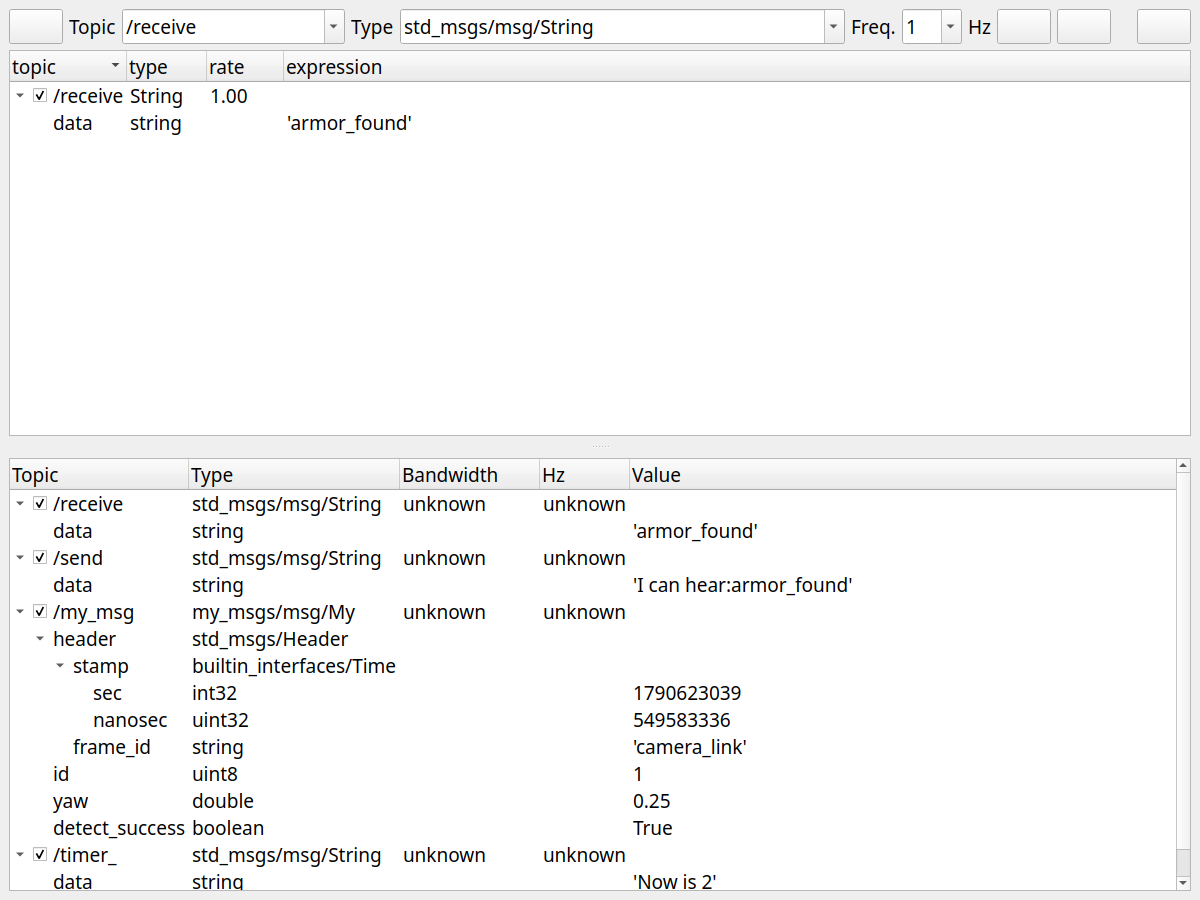
\includegraphics[width=0.8\textwidth]{ros2_rqt_revised.png}
  \caption{rqt 发布与监视插件：对照 receive 的输入与 send 的回复}
  \label{fig:ros2-rqt}
\end{figure}

图\ref{fig:ros2-rqt}中，上半部分是发布输入，下半部分是监视结果。重点看两条 data：输入是 armor\_found，回复多了 I can hear:，这正是字符串回调做的事情。你的窗口摆放可以不同，字段与话题应对应得上。

现在按 Ctrl+C 停止 my\_node。发布端还能发送 receive，但 send 不再有新回复；监视器可能暂时保留最后一条数据。重新启动节点后，如果话题条目被移除了，就重新勾选监视，再确认回复恢复。
\end{example}

\begin{exercise}
\label{ex:v2-ros-reply}
保持完整工程中的节点运行，把输入 hello 换成 armor\_found；记录 receive、send 的消息类型与返回内容。停止节点后再发一次，说明“命令发出了消息”和“程序处理了消息”有什么区别。
\end{exercise}
